\documentclass[10pt]{article}\usepackage[margin=18mm]{geometry}\usepackage{graphicx}\usepackage{hyperref}\setlength{\parskip}{5pt}\setlength{\parindent}{0pt}\title{Stage VI-0: Hierarchical Physical World-Model Validation}\author{Strictly offline local smoke validation}\date{2026-07-12}\begin{document}\maketitle\section{Decision}Decision C - descriptor schema still incomplete is the single main decision. The hierarchy resolves invalid-field mixing, but the full schema and uncertainty gates are not yet validated.\section{Scope}Frozen V3/V4 CSVs only. No exact solver, Delta-q search, active learning, HPC, or data edit. No learned state is transferable.\section{Hierarchy}Level 1 models SC existence and thermodynamics. Level 2 models the SC branch. Level 3 models trusted spectra. Level 4 models trusted gapped-SC Pfaffian outputs. Phase/topology labels are evaluation-only.\section{Matched smoke results}The mean spatial SC AUROC is 0.979. Median spatial $R^2$ is 0.441 for Level 1, 0.797 for Level 2, 0.051 for Level 3, and 0.912 for Level 4. Thermodynamics and $|q|$ are learnable. $P_0/P_\pi$ are learnable after trusted-gapped conditioning, but log-gap, $k_{gap}$, Pfaffian margin, and uncertainty-error alignment remain weak. Hierarchical Level-3 NLL improves over the same-split unified model; Level-4 improvement is not universal. Probe uncertainty is not monotonic across all run/level trajectories.\section{Critical answers}Thermodynamics can be learned independently. Conditioning makes $q$ learnable, but $\Delta F_{UF}$ cannot be tested. Topology regression becomes meaningful after invalid points are removed, yet its uncertainty is not consistently calibrated. The remaining failures are not mask sparsity alone because the spatial spectral/topology tests contain 639--694 valid points.\section{Caveat}The common frozen schema has no reliable $\Delta F_{UF}$ field.\clearpage\begin{figure}[p]\centering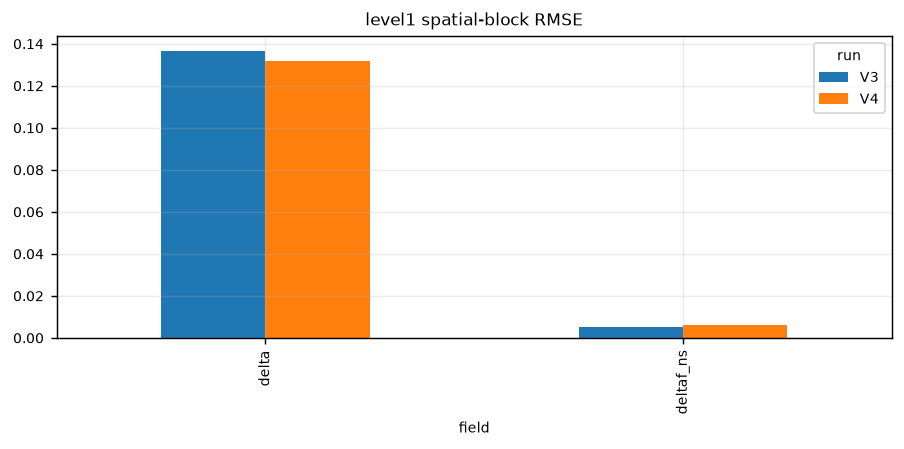
\includegraphics[width=.92\textwidth]{../figures/figure_01_level1_thermodynamics.png}\caption{figure 01 level1 thermodynamics}\end{figure}
\begin{figure}[p]\centering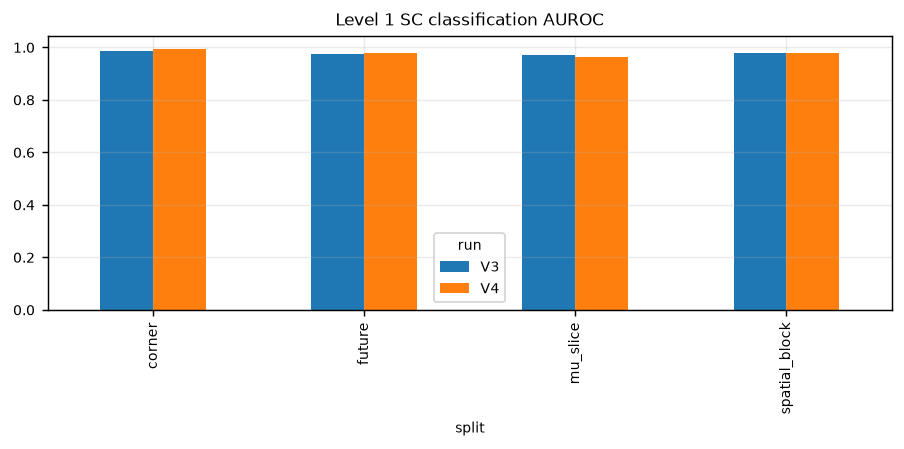
\includegraphics[width=.92\textwidth]{../figures/figure_02_level1_classification.png}\caption{figure 02 level1 classification}\end{figure}
\begin{figure}[p]\centering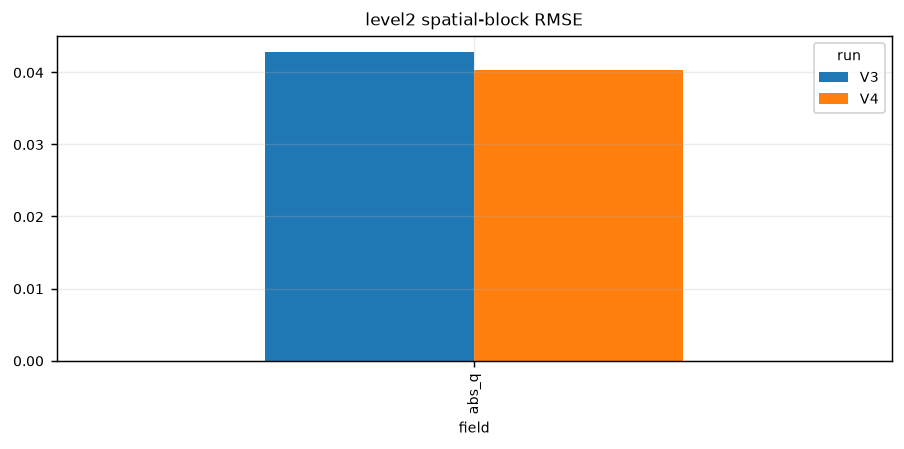
\includegraphics[width=.92\textwidth]{../figures/figure_03_level2_branch.png}\caption{figure 03 level2 branch}\end{figure}
\begin{figure}[p]\centering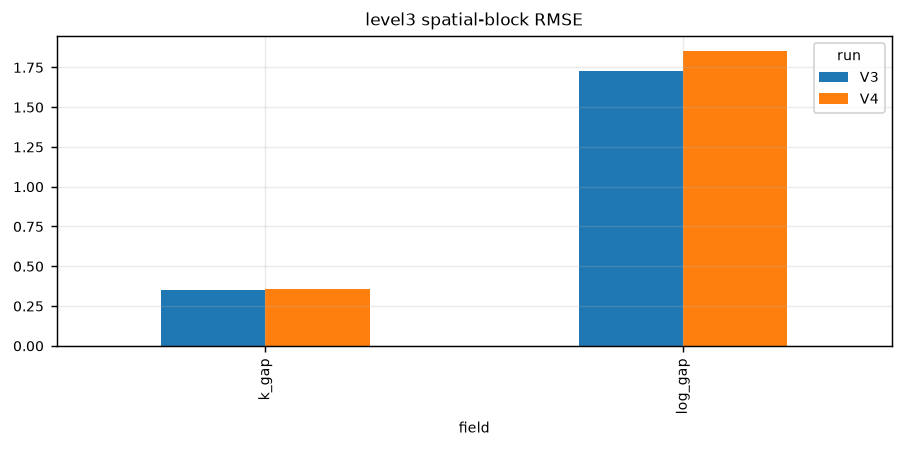
\includegraphics[width=.92\textwidth]{../figures/figure_04_level3_spectral.png}\caption{figure 04 level3 spectral}\end{figure}
\begin{figure}[p]\centering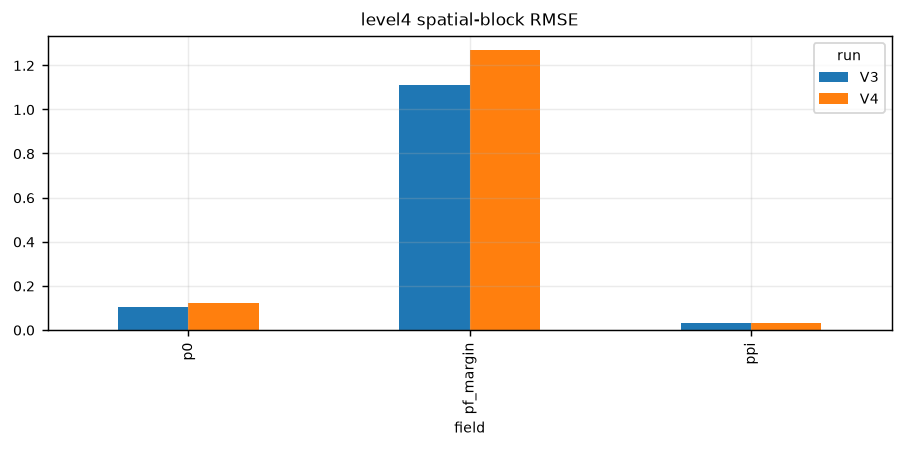
\includegraphics[width=.92\textwidth]{../figures/figure_05_level4_topology.png}\caption{figure 05 level4 topology}\end{figure}
\begin{figure}[p]\centering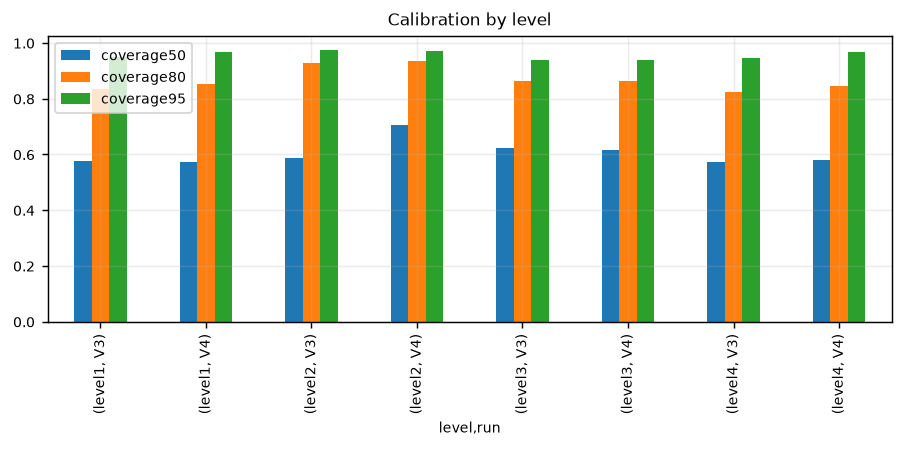
\includegraphics[width=.92\textwidth]{../figures/figure_06_calibration_by_level.png}\caption{figure 06 calibration by level}\end{figure}
\begin{figure}[p]\centering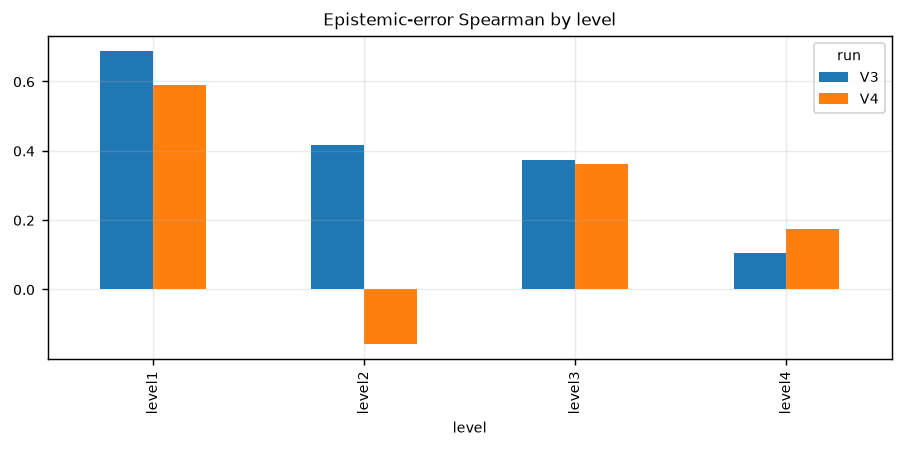
\includegraphics[width=.92\textwidth]{../figures/figure_07_uncertainty_error_by_level.png}\caption{figure 07 uncertainty error by level}\end{figure}
\begin{figure}[p]\centering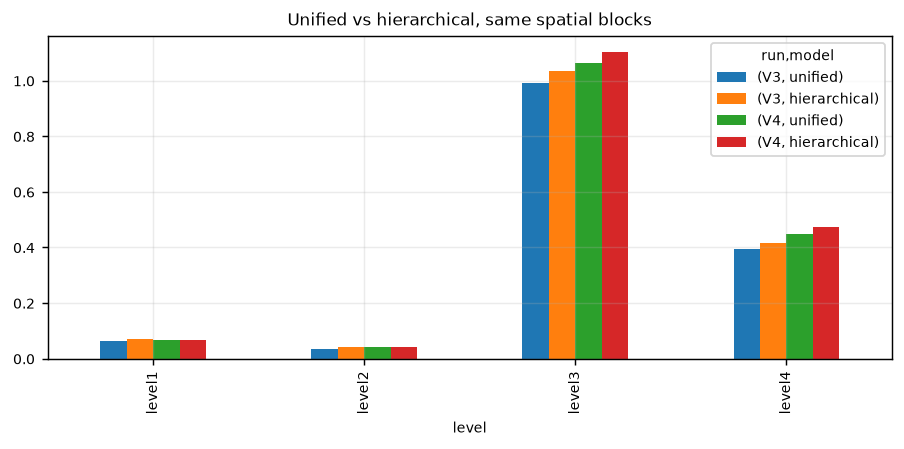
\includegraphics[width=.92\textwidth]{../figures/figure_08_unified_hierarchical.png}\caption{figure 08 unified hierarchical}\end{figure}
\begin{figure}[p]\centering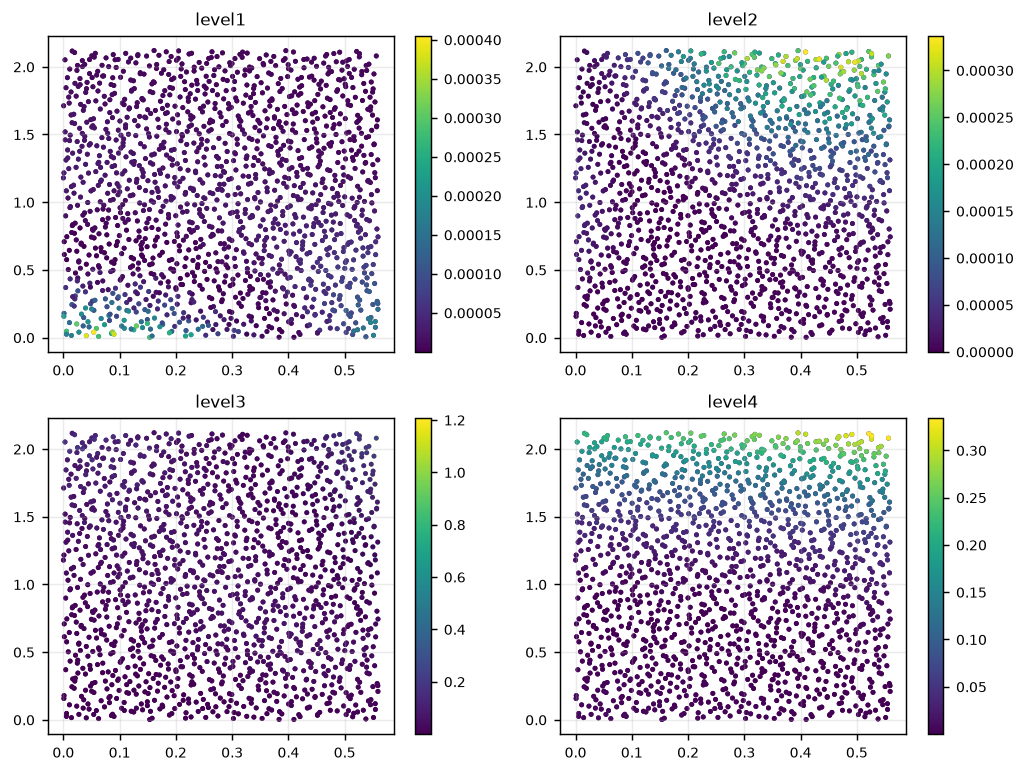
\includegraphics[width=.92\textwidth]{../figures/figure_09_probe_maps.png}\caption{figure 09 probe maps}\end{figure}
\begin{figure}[p]\centering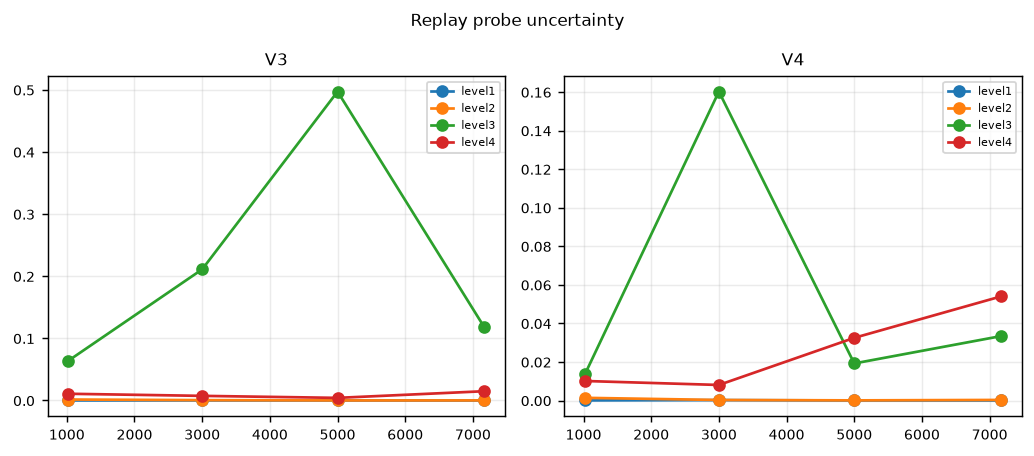
\includegraphics[width=.92\textwidth]{../figures/figure_10_replay_uncertainty.png}\caption{figure 10 replay uncertainty}\end{figure}
\begin{figure}[p]\centering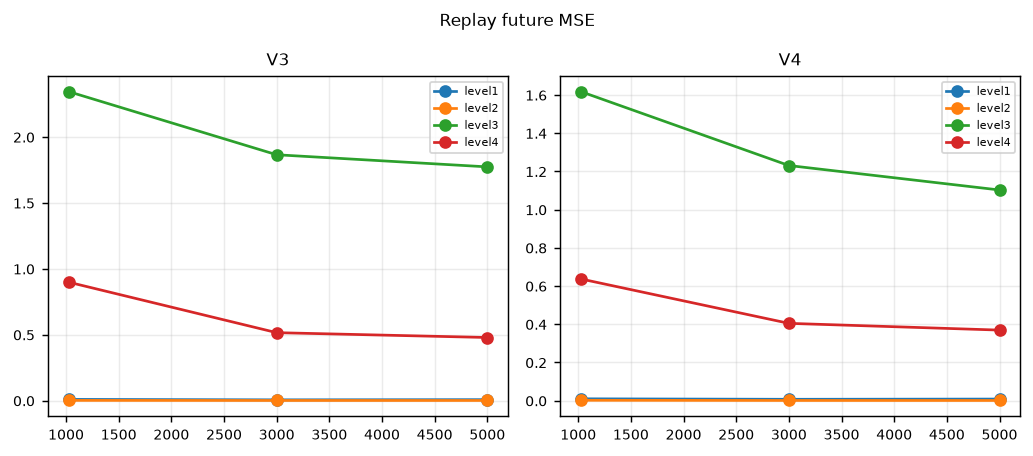
\includegraphics[width=.92\textwidth]{../figures/figure_11_replay_future_error.png}\caption{figure 11 replay future error}\end{figure}
\begin{figure}[p]\centering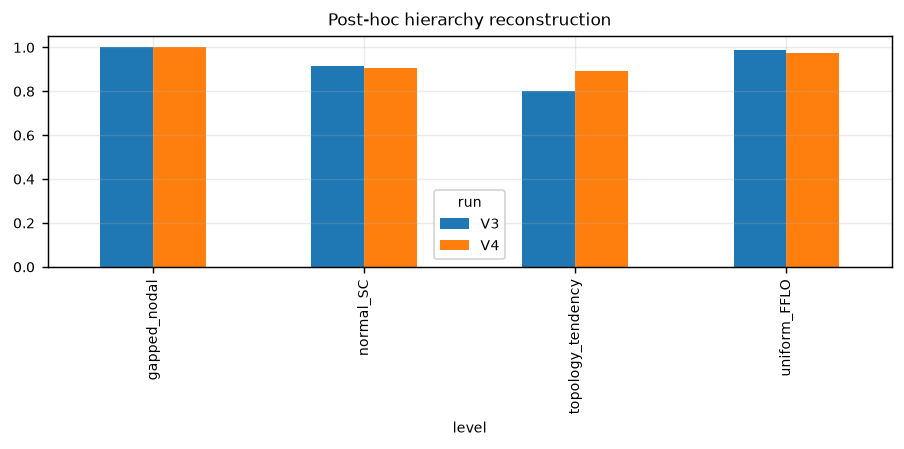
\includegraphics[width=.92\textwidth]{../figures/figure_12_phase_reconstruction.png}\caption{figure 12 phase reconstruction}\end{figure}
\begin{figure}[p]\centering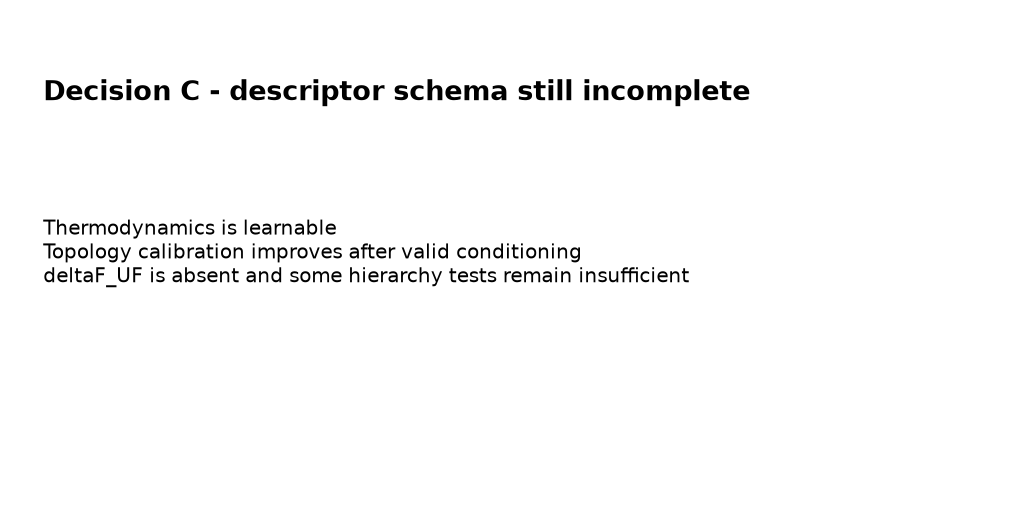
\includegraphics[width=.92\textwidth]{../figures/figure_13_decision.png}\caption{figure 13 decision}\end{figure}
\clearpage\section{Isolation}Only schema, masks, fixed transforms, architecture/loss source, validation source, and tests may be reused. All learned state is denied.\end{document}